\documentclass{article}
\usepackage[UTF8]{ctex}  % 使用中文支持包
\usepackage[a4paper, margin=1in]{geometry}  % 设置纸张大小和边距
\usepackage{anyfontsize}  % 解决字体大小报错问题
\usepackage{fancyhdr}  % 设置页眉、页脚、页码
\usepackage{lscape}
\usepackage{longtable}  % 支持长表格
\usepackage{booktabs}
\usepackage{graphicx}
\usepackage{colortbl}
\usepackage{graphicx}
\usepackage{tabularx}
\usepackage{multirow}
\usepackage[table,xcdraw]{xcolor}

\usepackage{amsmath}  % 数学公式支持
\usepackage{cases}  % 支持联立编号
\usepackage[sort]{natbib}  %国标参考文献 with sorting option

\usepackage{graphicx}  % 插入图片支持
\usepackage{float}  % 设置图片浮动位置
\usepackage{subfigure}  % 插入多图时用子图显示

\usepackage{listings}  % 代码块支持
\usepackage{xcolor}  % 设置代码块颜色

\lstset{
    basicstyle          =   \sffamily,          % 基本代码风格
    keywordstyle        =   \bfseries,          % 关键字风格
    commentstyle        =   \rmfamily\itshape,  % 注释的风格,斜体
    stringstyle         =   \ttfamily,  % 字符串风格
    flexiblecolumns,                % 别问为什么,加上这个
    numbers             =   left,   % 行号的位置在左边
    showspaces          =   false,  % 是否显示空格,显示了有点乱,所以不现实了
    numberstyle         =   \zihao{-5}\ttfamily,    % 行号的样式,小五号,tt等宽字体
    showstringspaces    =   false,
    captionpos          =   t,      % 这段代码的名字所呈现的位置,t指的是top上面
    frame               =   lrtb,   % 显示边框
}

\lstdefinestyle{Python}{
    language        =   Python, % 语言选Python
    basicstyle      =   \zihao{-5}\ttfamily,
    numberstyle     =   \zihao{-5}\ttfamily,
    keywordstyle    =   \color{blue},
    keywordstyle    =   [2] \color{teal},
    stringstyle     =   \color{magenta},
    commentstyle    =   \color{red}\ttfamily,
    breaklines      =   true,   % 自动换行,建议不要写太长的行
    columns         =   fixed,  % 如果不加这一句,字间距就不固定,很丑,必须加
    basewidth       =   0.5em,
}

\usepackage[hyphens]{url}  % 支持链接换行
\usepackage{hyperref}  % 超链接支持

\hypersetup{
    hidelinks,
    colorlinks=true,
    allcolors=black,
	pdfstartview=Fit,
	breaklinks=true
}

\usepackage{gbt7714}  %国标参考文献

\bibliographystyle{gbt7714-numerical}

\usepackage{lastpage}  % 添加lastpage包

\newcommand\f[2]{\frac{#1}{#2}}
\newcommand\pf[2]{\frac{\partial#1}{\partial#2}}
\newcommand\df[2]{\dfrac{#1}{#2}}
\newcommand\pdf[2]{\dfrac{\partial#1}{\partial#2}}
\newcommand\zsin[1]{\frac{e^{i#1}-e^{-i#1}}{2i}}
\newcommand\zdsin[1]{\dfrac{e^{i#1}-e^{-i#1}}{2i}}
\newcommand\zcos[1]{\frac{e^{i#1}+e^{-i#1}}{2i}}
\newcommand\zdcos[1]{\dfrac{e^{i#1}+e^{-i#1}}{2i}}
\newcommand\zline[1]{#1-\overline{#1}}
\newcommand\dg[2]{#1^{\circ}#2'}

\setlength{\headheight}{16pt}
\pagestyle{fancy}
\fancyhf{}

\title{\bf\huge 综述一种新型反应堆-沸水堆}
\author{Jerry}
\date{\today}
\pagenumbering{arabic}

\begin{document}

\fancyhead[L]{Jerry}
\fancyhead[C]{综述一种新型反应堆-沸水堆}
\fancyhead[R]{核电厂系统与设备-黄善仿}
\fancyfoot[C]{\thepage}

\maketitle

\section*{摘要}
本文探讨了先进沸水反应堆(ABWR)的发展及其在核能领域的应用,并详细介绍了ABWR的基本原理、主要结构和安全分析,展示了其在核能利用中的潜力和优势。ABWR结合了现代化技术,通过计算机控制和强化核安全措施,提高了反应堆的性能和安全性。ABWR反应堆采用轻水作为冷却剂和减速剂,使其适用于核电站发电、热电联产、海水淡化等多种场景。
\subsubsection*{关键词: 1. 沸水堆; 2. 核反应堆; 3. 核电厂}

\section{引言}

沸水反应堆(Boiling Water Reactor,简称BWR)是一种采用轻水作为冷却剂和减速剂的核电站发电装置。BWR的一种现代化改进设计被命名为先进沸水反应堆(Advanced Boiling Water Reactor,简称ABWR)。ABWR的研发始于20世纪80年代末至90年代初期,并随着时间的推移不断进行技术优化与升级。

ABWR的设计理念融合了多项先进技术,包括但不限于计算机控制系统、工厂自动化技术、控制棒的远程操控(移除、移动和插入)、堆芯循环水泵技术以及强化核安全措施。这些技术的集成应用,显著提升了原始BWR系列产品的性能,使得ABWR在保持高功率输出的同时(每台反应堆可达1350兆瓦),大幅降低了堆芯损坏的风险。尤为关键的是,ABWR采纳了全面标准化的设计理念,便于实现规模化生产,从而降低建设成本并缩短建设周期。

本研究旨在通过深入调研,了解沸水反应堆的应用场景、基本工作原理、主要结构与参数,以及在电力生产中的安全分析,以期为进一步推动我国核能技术的发展和核电站的安全高效运行提供理论依据和实践指导。

\section{应用场景}

先进沸水堆(如 ABWR )是核能技术发展的前沿,其在核电站发电、轻水堆技术发展、核能利用多样化等方面都展现出巨大的潜力。ABWR 进一步简化了设计,降低了成本,并提高了安全性和可靠性,使其成为未来核能发展的重要方向。它可以用于核电站发电,满足大规模电力需求,并具备良好的负荷跟随能力,适应电网负荷变化。先进反应堆已不仅仅局限于发电,而是得到了更为广泛的利用。如提供区域供热、工业供热、海水淡化,石油热采等等。其中核能供热尤其得到了快速发展。此外,ABWR 还可以用于海水淡化、核潜艇等多种核能利用场景,为人类提供清洁、可靠的能源,并推动核能技术的持续发展。\cite{kreithMECHANICALAEROSPACEENGINEERING}\cite{ChenJing600MWXiaoXingXianJinFeiShuiDuiGaiNianSheJiPdf1999}\cite{stosicBoilingWaterReactor2008}

目前,通用电气日立核能公司(GEH)和东芝公司提供ABWR。ABWR通过蒸汽驱动涡轮机,涡轮机连接发电机,从而产生电力;蒸汽通过核燃料中的裂变反应产生的热量从水中蒸发。柏崎刈羽核电站6号机组被认为是世界上第一座第三代反应堆。正在部署或运行的ABWR如表\ref{tab:abwr-now}:

\begin{table}[ht]
    \centering
    \resizebox{\columnwidth}{!}{%
        \begin{tabular}{@{}lll@{}}
        \toprule
        Plant Name & Rated Capacity & Location \\ \midrule
        Kashiwazaki-Kariwa Nuclear Power Plant & 1356 MW & Kashiwazaki, Japan \\
        Shika Nuclear Power Plant & 1358 MW & Shika, Japan \\
        Hamaoka Nuclear Power Plant & {\color[HTML]{323232} 1267 MW} & {\color[HTML]{323232} Omaezaki, Japan} \\
        Shimane Nuclear Power Plant Reactor 3 & {\color[HTML]{323232} 1373 MW} & {\color[HTML]{323232} Matsue, Japan} \\
        Lungmen Nuclear Power Plant & 1350 MW & Gongliao Township, Republic of China(Taiwan) \\
        Higashidōri Nuclear Power Plant & 1385 MW & Higashidōri, Japan \\
        Ōma Nuclear Power Plant & 1383 MW & Ōma, Japan \\
        South Texas Project & 1358 MW & Bay City, Texas, United States \\ \bottomrule
        \end{tabular}%
    }
    \caption{目前正在部署或运行的ABWR}
    \label{tab:abwr-now}
\end{table}

\section{基本原理}

沸水反应堆(BWR)采用铀氧化物(UO2)陶瓷作为燃料元件,这些燃料棒被封装在耐高压的锆合金包壳内,形成燃料组件,亦称为反应堆堆芯。在BWR中,轻水(普通水)不仅作为冷却剂,还充当中子慢化剂的角色。在堆芯内,快中子与铀-235发生核裂变反应,释放出次级中子,进而维持持续的链式反应。鉴于轻水的热中子吸收截面较大,必须通过插入含有硼或镉等中子吸收材料的控制棒来调节反应堆内的中子通量,确保反应堆的临界状态和稳定运行。\cite{dunbarBoilingWaterReactors2024}

BWR的工作原理涉及核裂变链式反应和热能转换两个主要阶段。在反应堆堆芯区域,核裂变产生的热能使冷却剂达到饱和状态并产生蒸汽。这些饱和蒸汽直接驱动汽轮机,进而带动发电机进行电能转换。在此过程中,蒸汽的质量流量大约为13\%,经过汽轮机膨胀做功后,蒸汽在冷凝器中被冷却成水,随后通过主给水泵重新送入反应堆压力容器,形成一个闭合的循环回路。尽管这种直接循环设计简化了热力系统,但也存在蒸汽发生器系统放射性污染的风险。在堆芯,冷却剂在维持适当的压力-温度条件下沸腾,产生驱动汽轮机的蒸汽。\cite{robinIntroductionNuclearReactors}

反应堆压力容器构成了反应堆冷却剂系统的压力边界,它不仅容纳堆芯,还负责固定和保持燃料组件及控制棒的准确位置,同时为冷却剂流动提供必要的通道。反应堆的控制操作是通过操纵控制驱动机构,实现控制棒在堆芯内的精准插入或抽出,以调节中子经济性。控制棒的中子吸收特性允许操作员精确控制反应堆功率水平,通过增加或减少可用于维持链式反应的中子数量,从而启动、维持或停止核裂变过程。\cite{robinIntroductionNuclearReactors}


\section{主要结构(参数)}

反应堆的主要结构包括反应堆容器、堆芯、控制棒、冷却剂循环系统、蒸汽发生器、蒸汽涡轮机、冷凝器等。沸水堆的主要结构包括以下几个关键部分:\cite{ChenJing600MWXiaoXingXianJinFeiShuiDuiGaiNianSheJiPdf1999}\cite{ChenJingXiaoXingJianHuaFeiShuiDuiYanJiuPdf2003}
\begin{itemize}
    \item \textbf{反应堆容器}:这是整个反应堆的核心部分,通常由耐腐蚀的不锈钢制成,形状为圆柱形,顶部开口以便于燃料组件的插入和更换。反应堆容器内部装有反应堆堆芯,即燃料组件。
    \item \textbf{燃料组件}:燃料组件是沸水堆中非常重要的部分,它们由许多细长的管子组成,管内填充有核燃料(通常是低 enriched uranium 或 high enriched uranium)。这些燃料棒在反应堆中进行核裂变,释放出能量。
    \item \textbf{冷却剂系统}:在沸水堆中,冷却剂(通常是水)直接通过反应堆容器底部进入,吸收反应堆产生的热量并将其带出。冷却剂在反应堆容器内沸腾,产生蒸汽。
    \item \textbf{蒸汽发生器}:虽然在传统的沸水堆中冷却剂直接产生蒸汽,但在一些改进型沸水堆(如ABWR)中,蒸汽发生器被用来进一步提高效率。蒸汽发生器将冷却剂的热能传递给二次侧的水,使其沸腾产生蒸汽。
    \item \textbf{控制系统}:控制系统用于监控和调节反应堆的运行状态,包括控制棒的插入和抽出以调节反应性,以及调节冷却剂的流量和温度。
    \item \textbf{安全系统}:包括紧急冷却系统、辐射防护系统等,确保在异常情况下能够迅速有效地保护反应堆和周围环境。
\end{itemize}

对于具体的参数,以SSBWR-200反应堆为例,主要参数如表\ref{tab:ssbwr_200_main_parameters}所示。\cite{ChenJingJianHuaFeiShuiDuiSSBWR200DeReGongSheJiHeShiGuFenXi2001}

\begin{table}[ht]
    \centering
    \caption{SSBWR-200 主要参数}
    \label{tab:ssbwr_200_main_parameters}
    \begin{tabular}{llll}
        \toprule
        项目 & 参数 & 项目 & 参数 \\
        \midrule
        热功率 & 630 MW & 电功率 & 30~300 MW \\
        供热 & 0~500 MW & 寿命 & 60 a \\
        蒸汽温度 & 286 ℃ & 蒸汽压力 & 7.0 MPa \\
        堆芯有效高度 & 2.2 m & 堆芯有效直径 & 3.48 m \\
        堆芯体积功率密度 & 30 kW/L & 燃料组件数目 & 384 个 \\
        控制棒数目 & 89 根 & 压力壳(RPV)内直径 & 5 m \\
        压力壳(RPV)高度 & 18 m & 安全壳内直径 & 35 m \\
        安全壳高度 & 22 m & 蒸汽流量 & 1.226 kt·h$^{-1}$ \\
        堆芯冷却剂流量 & 15.95 kt·h$^{-1}$ & 给水流量 & 1.226 kt·h$^{-1}$ \\
        堆芯传热总面积 & 2521 m$^{2}$ & 堆芯入口温度 & 280.7 ℃ \\
        给水温度 & 216.8 ℃ & 堆芯平均空泡份额 & 38.0 \% \\
        堆芯出口平均含汽率 & 5.8 \% & 最小临界功率比(MCPR) & $>$2.5 \\
        平均线功率密度 & 7.85 kW·m$^{-1}$ & 最大线功率密度(MLHGR) & 23.7 kW·m$^{-1}$ \\
        \bottomrule
    \end{tabular}
\end{table}

\section{安全分析}

\subsection{堆芯安全分析}

ABWR为了保证堆芯不发生熔化,设置了反应堆应急冷却剂(ECCS);为了防止核废料物质超标释放到环境中,设置了反应堆安全壳系统。由应急堆芯冷却系统和安全壳系统组成了先进沸水堆安全系统,可有效冷却堆芯和堆内构件,避免发生堆芯碎片及裂变产物泄漏到环境系统结构如以ABWR为例,如图\ref{fig:abwr-security}所示。从以ABWR为例,如图\ref{fig:abwr-security}可知。先进沸水堆安全系统主要由应急堆芯冷却系统(ECCS)和安全壳系统组成。应急堆芯冷却系统基本功能是:当先进沸水堆的一回路系统管道破裂后,引起失水事故时为先进沸水堆提供冷却剂,能确保堆芯始终处于淹没状态,维持堆芯冷却。应急堆芯冷却系统由堆芯隔离冷却系统(RCIC)、高压堆芯注水系统(HPCF)、余热排出系统(RHR)的低压注水运行模型(LPFL)组成,自动降压系统(ADS)作为备用。应急堆芯冷却系统分为3个功能区域:区域I由堆芯隔离冷却系统(RCIC)、1个余热排出系统(RHR)的低压注水运行模型(LPFL)、自动降压系统(ADS)组成:区域II由1个高压堆芯注水系统(HPCF)、1个余热排出系统(RHR)的低压注水运行模型(LPFL)、自动降压系统(ADS)组成:区域III由1个高压堆芯注水系统(HPCF)、1个余热排出系统(RHR)的低压注水运行模型(LPFL)、自动降压系统(ADS)组成。当先进沸水堆出现事故,发出信息,应急堆芯冷却系统各系统触发信号,相互配合共同完成应急堆芯冷却系统功能。安全壳系统主要由安全壳、安全壳排热系统、安全壳隔离系统、安全壳内可燃性气体控制系统等组成。其中先进沸水堆安全壳采用可拆卸钢封头的压力抑制型钢筋混泥土结构;当先进沸水堆发生失水事故时,由安全壳排热系统(CHriS)防止安全壳超温、超压,保证先进沸水堆完整性。\cite{ChenJieChaoLinJieShuiDuiYuXianJinFeiShuiDuiAnQuanTeXingChaiYiXingFenXi2016}

\begin{figure}[ht]
    \centering
    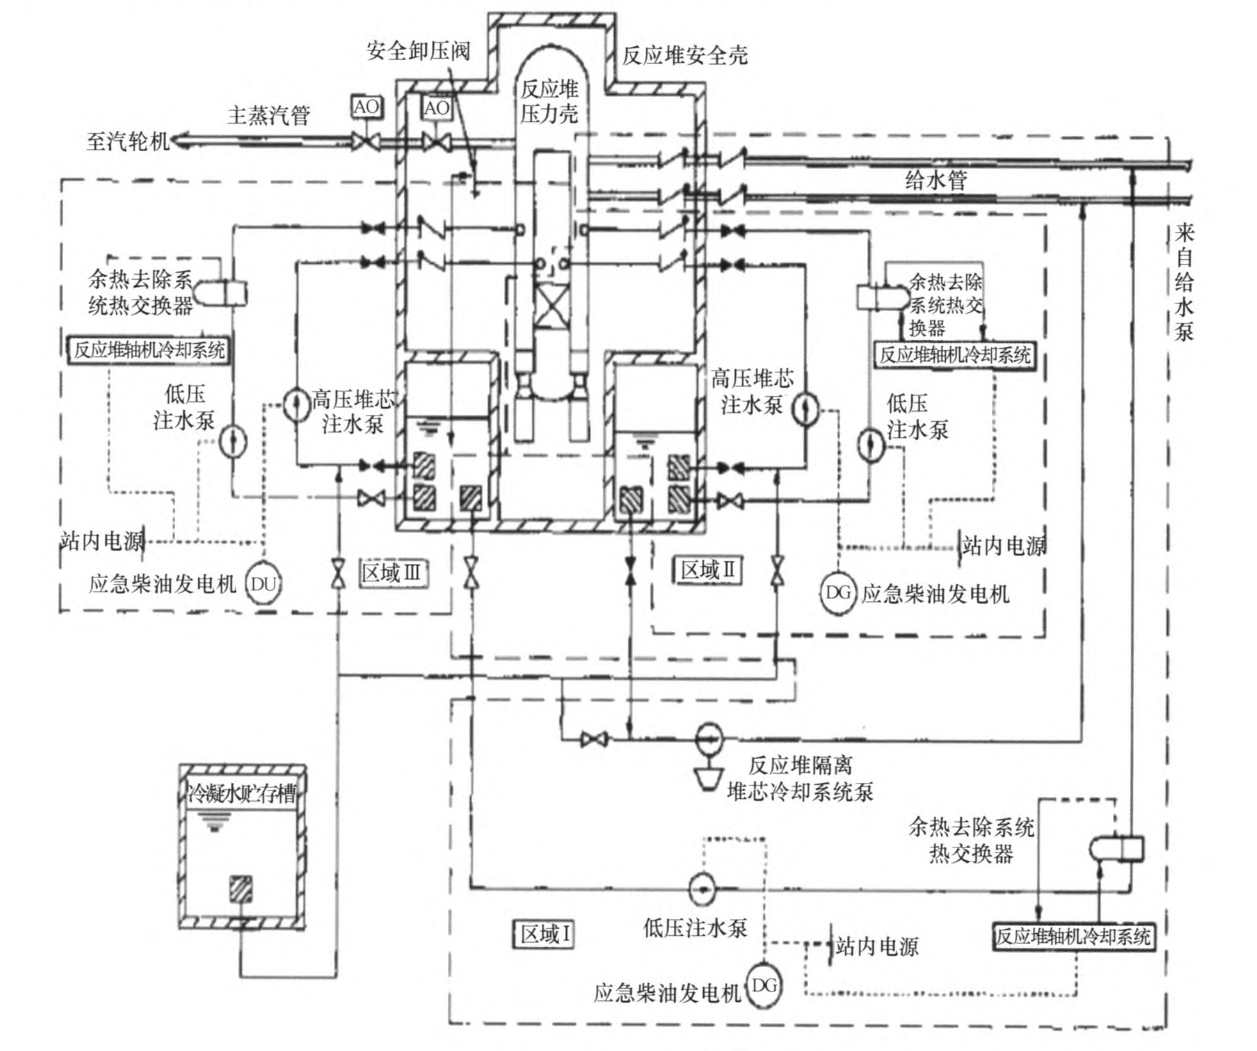
\includegraphics[width=0.8\textwidth]{figures/Security System of ABWR.png}
    \caption{先进沸水堆安全系统}
    \label{fig:abwr-security}
\end{figure}

\subsection{主控室安全分析}

对于主控室方面(人因因素),ABWR相对于BWR有了以下的改进\cite{LiuXinRongXianJinFeiShuiDuiABWRDeTeXingYuKeYongXing1996}

\begin{table}[ht]
    \centering
    \caption{ABWR和BWR主控室的比较}
    \resizebox{\columnwidth}{!}{%
        \begin{tabular}{|p{2.5cm}|p{4.8cm}|p{4.8cm}|}
        \hline
        & BWR & ABWR \\
        \hline
        面积 & 大 & 明显减小 \\
        \hline
        技术 & 模拟控制、硬线 & 数字控制、光纤传输 \\
        \hline
        大模拟盘 & 无 & 有,全厂监察工业电视 \\
        \hline
        控制器 & 分别为各工艺设备采用单一硬线连接开关 & 为触摸式CRT,平板控制器,系统级控制 \\
        \hline
        控制台的显示 & 专用硬显示器 & CRT平板显示器 \\
        \hline
        操作员 & 约4人(典型的) & 约3人 \\
        \hline
        人因工程 & 三哩岛事件后作局部改进 & 设计中全盘考虑 \\
        \hline
        \multirow{6}{*}{操纵员支持手段} & 书面规程 & CRT显示规程 \\
            & 手动操作 & 根据要求自动操作、快速的菜单驱动 \\
            & 复杂的技术规格书 & 计算机监测和显示实时参数以及运行限值和运行条件 \\
            & 书面的应急运行规程 & 应急规程专家系统在CRT上给出运行指导 \\
            & 安全参数显示系统是三哩岛事件后增设的 & 安全参数显示系统是作为信息系统的一项功能统一考虑的。 \\
        \hline
    \end{tabular}
  }
\end{table}

\subsection{对于简化沸水堆的设计更新的分析}

\textbf{采用自然循环:}自然循环是最重要的非能动安全设计。在以前的小型实验堆中采用的比较多,但在动力 堆中主回路采用自然循环的很少。在新一代先进小型沸水堆设计中,一回路全部采用自然循环。,绝大部分余热冷却、堆芯紧急冷却、安全壳冷却也采用非能动的自然循环。这样的设计使BWR比以前的动力堆具有更好的安全性,同时系统更为简化,较好地实现了安全和经济的统一。

\textbf{采用大水池结构:}大型的水池具有很大的热容量,能有效地抑制事故情况下压力与温度的上升,在新一代沸水堆设计中用得特别多。水池结构在传统的BWR中也是常规的设计,但都只是起单一的抑压功能。在简化沸水堆设计中,水池除了抑压作用以外,同时还起非能动的堆芯紧急冷却,或余热冷却,或安全壳冷却等多种作用,而且其位置大都由压力容器底部提升到堆芯高度以上。水池结构的巧妙使用是SBWR区别于传统BWR的关键所在,也是SBWR实现非能动安全功能的主要设计。

\textbf{改进安全壳型式及其冷却:}安全壳是反应堆系统的最后一道安全屏障,也是造价最昂贵的部件之一。对它的改进在安全上带来的好处和经济上的节省是十分明显的。因此,SBWR设计重视安全壳的改进, 提出了一些独特的设计,如GESBWR的小型抑压安全壳及其非能动冷却系统,西门子SBWR200的包括附属设备及汽轮机在内的整体式安全壳等。\cite{YanYuHuaXinYiDaiJianHuaFeiShuiDuiHeDianZhanFaZhanGaiKuangJiQiTeDian1997}

\bibliography{cite.bib}

\vspace{3em}

{
\centering\textbf{\huge An overview of a new type of reactor - the boiling water reactor} \\
}

\section*{Abstract}

This article discusses the development of advanced boiling water reactors (ABWRs) and their applications in nuclear energy, and provides a detailed description of the basic principles, main structures, and safety analyses of ABWRs, demonstrating their potential and advantages in the utilization of nuclear energy.ABWRs incorporate modern technologies to improve reactor performance and safety through computer control and enhanced nuclear safety measures.ABWR reactors use light water as the coolant and decelerator, making it suitable for a wide range of scenarios, including nuclear power generation, cogeneration, and seawater desalination.

\subsubsection*{Keywords: 1. Boiling Water Reactor, 2. Nuclear Reactor, 3. Nuclear Energy, 4. Nuclear Power Plant, 5. Safety Analysis}

\end{document}